\chapter{Implemenations and Evaluations}

This chapter presents details of the implementations, experiments and evaluations for the proposed models in previous chapter. Section \ref{sec:chap4_implementation} describes the architecture of training system written in Torch framework which was used to train all the models. Before going onto detailed experiments and evaluations, section \ref{sec:chap4_metric} provides explanation for the metrics used to evaluate models' performances includeng BLUE, METEOR and CIDEr scores. Subsequently, section \ref{sec:chap4_experiment} presents all the experiments along with evaluation and assessment for each of them.

%% -------------------------------------
%% SECTION 1:
%%   Implementations
%% -------------------------------------
\section{Implementations}
\label{sec:chap4_implementation}


\subsection{Training System Architecture}

\subsection{Training and Monitoring}
Training a deep neural network can be very hard and time-consuming. During the course of training of all models and experiments presented in this thesis, I have followed several guidelines \cite{bottou-tricks-2012} on tips and tricks to effectively train deep neural networks.
	\subsubsection{Choosing a right learning rate}
	As shown in \cite{Murata98astatistical}, the mathematics of stochastic gradient descent do not depend on the size of training set. Therefore, the best way to determine the correct learning rates is to perform experiments on a small but representative traing set. When the model performs well on training cost with the sample training set with some learning rate $\gamma_t$, we can apply that learning rate to train our model on real training set.

	For this purpose, I set up a small experiment on subset of MSCOCO dataset (see \ref{sec:dataset_mscoco} for details). The subset COCO-1k consists of images randomly from MSCOCO training set. There are in total $1,200$ images in COCO-1k; $1,000$ of them are in training set and the rest are reserved in the validation set. I trained a model with 16-layer VGGNet as CNN; optimization method is SGD; the LSTM has 512 hidden units and with batch size equals to 5.
%% -------------------------------------
%% SECTION 2:
%%   Evaluation metrics
%% -------------------------------------
\section{Evaluation Metrics}
\label{sec:chap4_metric}
Even though there has not existed any clear methodology to decide whether a generated caption is deemed successful or not given an input images, researchers of image captioning and machine translation often use several methods to evaluate the quality of the captions. The most commonly used metric so far in the image caption literature has been the BLUE score \cite{Papineni:2002:BMA:1073083.1073135}. Though the metric has recently been critised due to some obvious drawbacks, it has been shown to correlate well with human evaluations. In addition, another scores which are also often used are METEOR and CIDer.

\subsection{BLUE}
Let \textit{c} be the length of the generated caption and \textit{r} be the length of the groundtruth caption in the dataset. The brevity penalty BP is computed as
\begin{align}
	BP &= \left\{
		\begin{tabular}{l l}
			1 & if $c > r$ \\
			$e^{\left(1 - r/c\right)}$ & if $c \leq r$
		\end{tabular}
	\right.
\end{align}
Then,
	\begin{tcolorbox}[ams align, colback=yellow!10!white,colframe=bordeuxcolor]
	% \begin{align}
		\centering
		\text{BLUE} &= \text{BP}.\text{exp}\left( \mathlarger{\sum^N_{n=1}}w_n\text{log}p_n\right) 
	% \end{align}
	\end{tcolorbox}
The ranking behavior is more immediately apparent in the log domain
\begin{align*}
	\text{log BLUE} &= \text{min} \left(1 - \frac{r}{c}, 0\right) + \mathlarger{\sum^N_{n=1}} w_n\text{log}p_n 
\end{align*}


\subsection{METEOR}
In the context of image captioning, METEOR \cite{denkowski:lavie:meteor-wmt:2014} is a language specific translation evaluation method for any target language. It evaluates the generated caption by aligning it to the groundtruth sentence and calculating sentence-level similarity scores.
The METEOR score for a sentence pair is calculated as follow:
\begin{itemize}
	\item Content and function words are identified in the hypothesis $\left(h_c, h_f\right)$ and reference $\left(r_c, r_f \right)$ according to a function word list

	\item For each of the matchers $\left( m_i \right)$ count the number of content and function words covered by matches of this type in the hypothesis $\left(m_i\left(h_c\right), m_i\left(h_f\right)\right)$ and reference $\left(m_i\left(r_c\right), m_i\left(r_f\right) \right)$

	\item Calculate weighted precision and recall using matcher weights $\left(w_i .s w_n\right)$ and content-function word weight $\left( \delta \right)$:
	\begin{align}
		P &= \frac{\sum_i w_i \cdot \left( \delta \cdot m_i\left(h_c\right) + \left(1 - \delta \right) \cdot m_i \left(h_f\right) \right)}{\delta \cdot |h_c| + \left( 1 - \delta \right) \cdot |h_f|} \\
		R &= \frac{\sum_i w_i \cdot \left( \delta \cdot m_i\left(r_c\right) + \left(1 - \delta \right) \cdot m_i \left(r_f\right) \right)}{\delta \cdot |r_c| + \left( 1 - \delta \right) \cdot |r_f|}
	\end{align}

	\item Calculate the harmonic mean of $P$ and $R$:
	\begin{align}
		F_{\text{mean}} = \frac{P . R}{\alpha . P + \left( 1 - \alpha \right) . R}
	\end{align}

	\item To account for gaps and differences in word order, a fragmentation penalty is calculated using the total number of matched word ($m$, averaged over hypothesis and reference) and number of chunks $\left(ch\right)$:
	\begin{align}
		\text{Pen} = \gamma . \left( \frac{m}{ch} \right) ^ \beta
	\end{align}

	\item The METEOR score is then calculated:
	\begin{tcolorbox}[ams align, colback=yellow!10!white,colframe=bordeuxcolor]
	% \begin{align}
		\centering
		\text{METEOR} = \left(1 - \text{Pen} \right) . F_{\text{mean}}
	% \end{align}
	\end{tcolorbox}
\end{itemize}


\subsection{CIDEr}
CIDEr (Consensus-Based Image Description Evaluation) \cite{DBLP:journals/corr/VedantamZP14a} is an novel paradigm for evaluating image captions using humn consensus. It automatically evaluate for image $I_i$ how well a candidate sentence $c_i$ matches the consensus of a set of image descriptions $S_i = \{s_{i1}, \dots, s_{im}\}$. Each sentence is presentation by a set of $n$-grams (typically $n \in \{1, 2, 3, 4\}$).

To calculate CIDEr score, we first have to perform a Term Frequency Inverse Document Frequency (TF-IDF) weighting for each $n$-grams. We compute the TF-IDF weighting $g_k\left(s_{ij}\right)$ for each $n$-gram $\omega_k$ using
\begin{align}
	g_k\left(s_{ij}\right) = \frac{h_k\left(s_{ij}\right)}{\sum_{\omega_l \in \Omega} h_l \left(s_{ij}\right)} \log \left( \frac{|I|}{\sum_{I_p \in I} \min \left( 1, \sum_q h_k \left(s_{pq} \right)\right)}  \right)
\end{align}
Then, CIDEr score is calculated as:
\begin{tcolorbox}[ams align, colback=yellow!10!white,colframe=bordeuxcolor]
	\centering
	\text{CIDEr}\left(c_i, S_i\right) &= \mathlarger{\sum_{n=1}^N} w_n \text{CIDEr}_n\left(c_i, S_i\right)
\end{tcolorbox}
In practice, $w_n = 1/N$ where $N = 4$ yields the best results

%% -------------------------------------
%% SECTION 3:
%%   Experimental Environment
%% -------------------------------------
\section{Experimental Environment}
\label{sec:chap4_environment}

\subsection{Hardware configurations}
All models are trained with the following hardware configurations:

\begin{table}
	\centering
	\label{tab:hardware_configuration}
	\caption{Hardware configuration for training all models}
	\begin{tabular}{|l|l|}
		\hline
		CPU & Intel(R) Xeon(R) E5-2620 (15MB cache, 2.40GHz) \\ \hline
		Memory & 128 GB \\ \hline
		GPU & 2 x nVidia Tesla K80 [GK210B], each with $2,496$ CUDA cores, $12$GB VRAM, 240 GB/s memory bandwidth \\ \hline
		Storage & 4TB \\ \hline
	\end{tabular}
\end{table}

\subsection{Datasets}
\subsubsection{Flickr8k}
Flickr8K was first proposed by \cite{Hodosh:2013:FID:2566972.2566993} as a benchmark collection for sentence-based image description and search. The dataset consists of $8,000$ images accompanied with five different description sentences which provide clear description of salient entities and events. \textit{TODO: re-paraphrase}
\subsubsection{Flickr30k}
As introduced in \cite{DBLP:journals/tacl/YoungLHH14}, Flickr30k is an extension of Flickr8k. The dataset is comprised of $158,915$ crowd-sourced captions describing $31,783$ images. Except for images that overlapped in Flickr8k, the new images and captions in this dataset focus on people involved in everyday activities and events.

Several examples of images and captions in Flickr8K and Flickr30k are shown in figure \ref{fig:flickr-examples}.

\begin{figure}
	\centering
	\label{fig:flickr-examples}
	\begin{tabular}{l l}
		\toprule
		\multirow{5}{*}{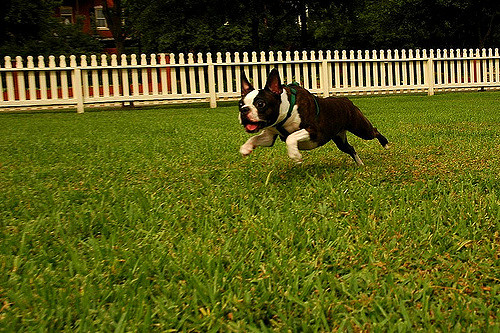
\includegraphics[width=0.25\linewidth]{Chapters/Fig/black_dog_running_fence.jpg}} & \parbox{11cm}{\small{A black and white dog is running in a grassy garden surrounded by a white fence}} \\
		& \small{A black and white dog is running through the grass} \\
		& \small{A Boston terrier is running in the grass} \\
		& \small{A Boston Terrier is running on lush green grass in front of a white fence} \\
		& \small{A dog runs on the green grass near a wooden fence} \\
		\midrule
		\begin{minipage}{0.25\linewidth}
			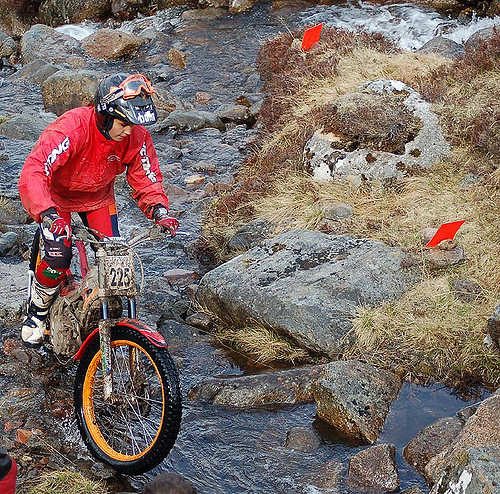
\includegraphics[width=\linewidth]{Chapters/Fig/men_red_helmet_riding_bike_rocks.jpg}
		\end{minipage}
		&
		\begin{minipage}{0.75\linewidth}
			\parbox{11cm}{\small{A boy in a black helmet and red long sleeve shirt rides his motorbike over a rocky stream}} \\
			\small{A man on a motorcycle steers through swampy terrain} \\
			\small{A man rides his bike over rocks and a creek.} \\
			\small{A motocross bike is being ridden between markers in a running stream.} \\
			\small{A person is dirt biking over rocks and water.}
		\end{minipage}\\
		\midrule
		\begin{minipage}{0.25\linewidth}
		IMAGE 335110163
			% \includegraphics[width=\linewidth]{Chapters/Fig/woman_photograph.png}
		\end{minipage}
		&
		\begin{minipage}{0.75\linewidth}
			\parbox{11cm}{\small{A woman with dark hair and a white shirt is taking a picture of an object at close range }} \\
			\parbox{11cm}{\small{A photographer taking a closeup photo of a glass perfume jar }} \\
			\parbox{11cm}{\small{A woman taking picture of her pet in her home }} \\
			\parbox{11cm}{\small{A woman taking a photo of an object on a bed }} \\
			\parbox{11cm}{\small{The lady is taking a closeup picture }} \\
		\end{minipage}\\
		\begin{minipage}{0.25\linewidth}
		IMAGE 908636680
			% \includegraphics[width=\linewidth]{Chapters/Fig/woman_photograph.png}
		\end{minipage}
		&
		\begin{minipage}{0.75\linewidth}
			\parbox{11cm}{\small{A group of eight campers sit around a fire pit trying to roast marshmallows on their sticks}} \\s
			\parbox{11cm}{\small{A group of men and women surrounding a bonfire while having conversation }} \\
			\parbox{11cm}{\small{Several people having fun and toasting marshmallows around a campfire }} \\
			\parbox{11cm}{\small{A group of people are outside , roasting marshmallows in a fire }} \\
			\parbox{11cm}{\small{Seven adults sit around a fire pit having a conversation }} \\
		\end{minipage}\\
		\bottomrule
	\end{tabular}
	\caption{Images with 5 crowd-sourced captions in Flickr8k and Flickr30k}
\end{figure}

\subsubsection{MSCOCO}
\label{sec:dataset_mscoco}

MSCOCO \cite{DBLP:journals/corr/LinMBHPRDZ14} (Microsoft Common Objects in Context) is a large-scale dataset that addresses three core research problems in scene understanding: detecting non-iconic views of objects, contextual reasoning between objects and the precise 2D localization of objects. It has been considered as the start-of-the-art dataset for numerous computer vision tasks (e.g., image classification, object detection, object segmentation, scene labelling, etc.). The dataset has approximately $328,000$ images of complex everyday scenes containing common objects in their natural context. Like in aforementioned Flickr8k \& Flickr30k datasets, each images in MSCOCO is also associated with five caption sentences that describe the content of such image.

The statistics of the datasets are summarized in table \ref{tab:dataset-statistics}
\begin{table}
	\centering
	\label{tab:dataset-statistics}
	\begin{tabular}{l|c|c|c}
		\toprule
		\multirow{2}{*}{Dataset name} & \multicolumn{3}{c}{size} \\ \cline{2-4}
		& train & validation & test \\ \midrule
		Flickr8k & 6000 & 1000 & 1000 \\
		Flickr30K & 28000 & 1000 & 1000 \\
		MSCOCO & 82783 & 40504 & 40775 \\
		\bottomrule
	\end{tabular}
	\caption{Dataset statistics}
\end{table}


%% -------------------------------------
%% SECTION 4:
%%   Experiments
%% -------------------------------------
\section{Experiments and Evaluations}
\label{sec:chap4_experiment}

\subsection{Experiment 1: The effects of different optimization methods}
